\chapter{}

\centerline{{\large An Interview With Prof.\ V.\ Ramgopal Rao.}}

\vskip .5cm

\noindent\makebox[\textwidth]{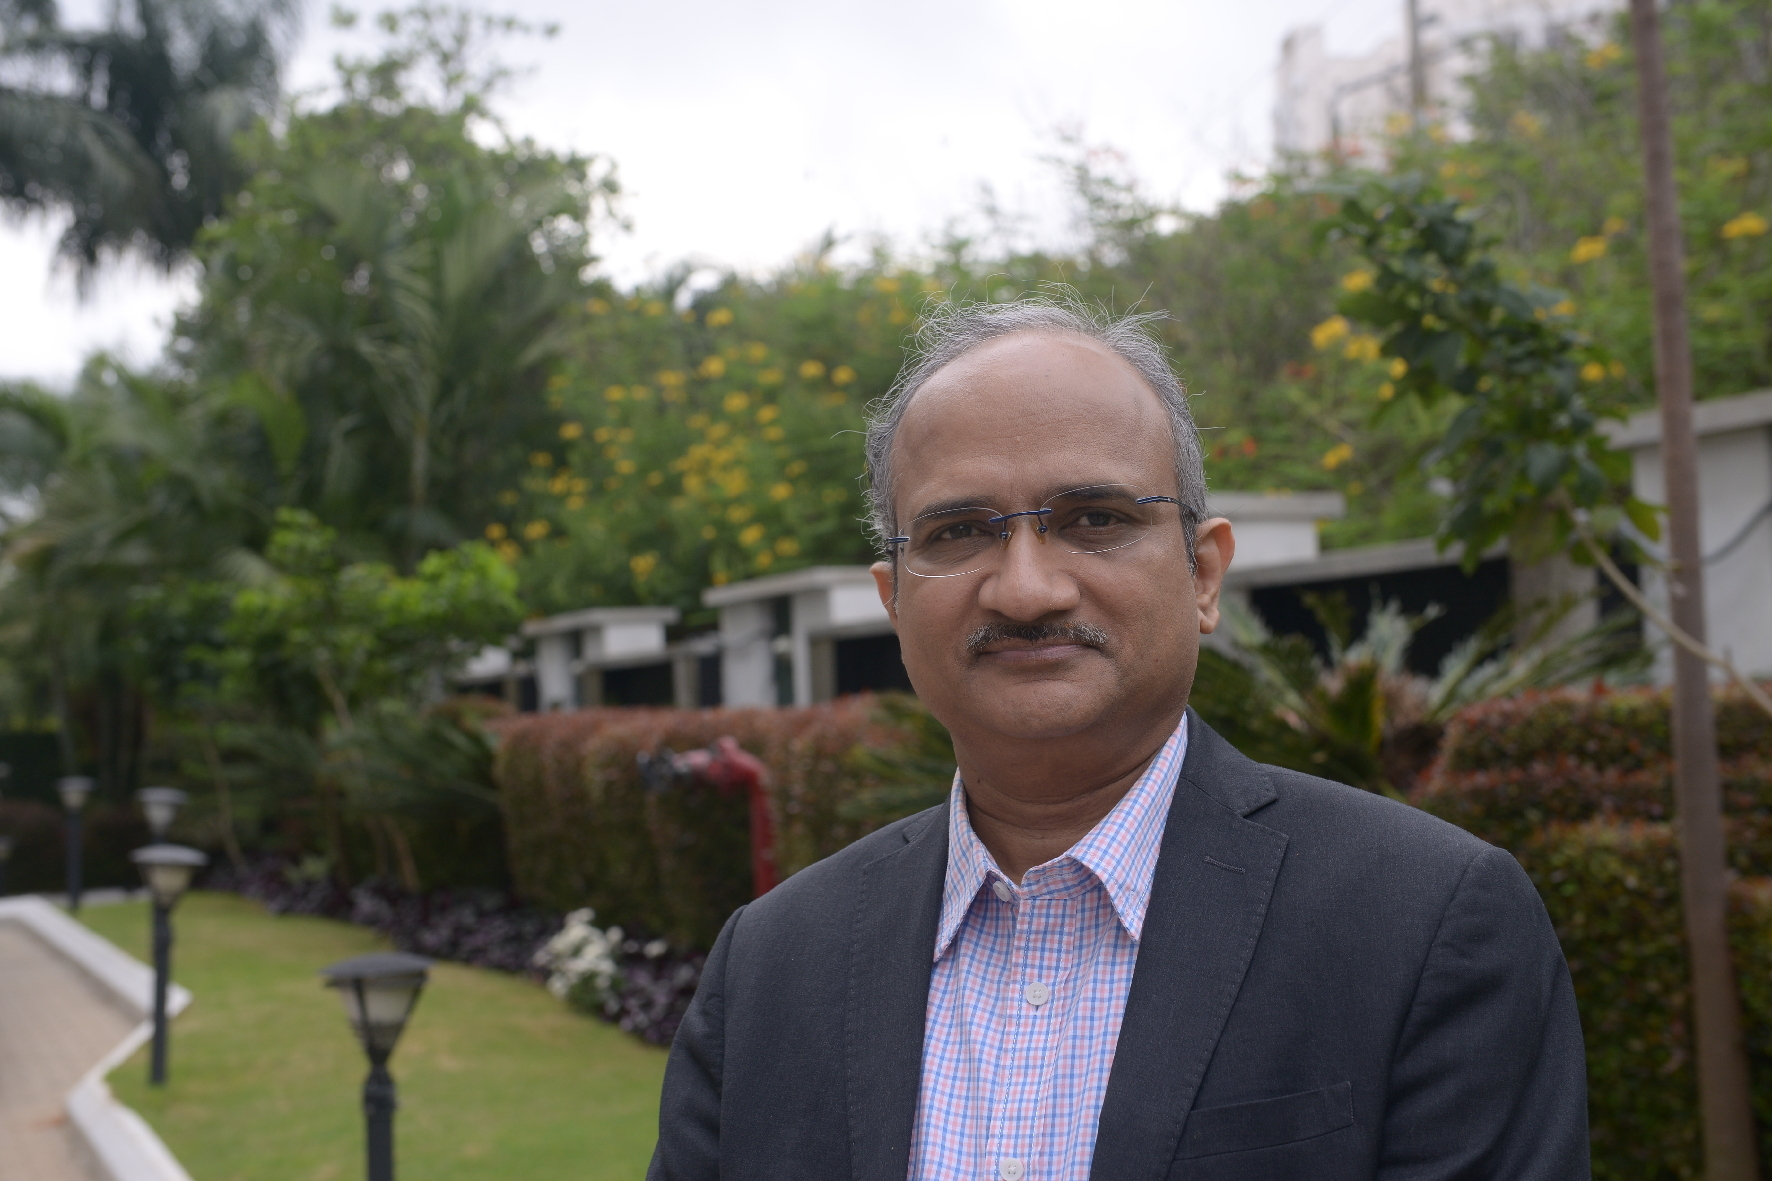
\includegraphics[width=\textwidth]{src/Figures/interview/interview-fig08.jpg}}

\vskip .85cm

\begin{multicols}{2}

\textbf{Prof. V Ramgopal Rao, is leading investigations into the science and engineering of nanoscale electronic devices. His seminal work on FinFeT transistors using bulk  CMOS instead of Silicon on Insulator (SoI) technology has led to further miniaturiation processors beyond 7 nm. Prof. Rao was conferred the ACCS-CDAC Award for 2019 at ADCOM 2019. Prashanth Hebbar from ACC Journal caught up with Prof Rao and discussed on a range of subjects close to the Prof. Rao’s heart. This is excerpt from the discussion.}

\textbf{Prashanth Hebbar (PH): how did you really get interested in MOSFETs? When you entered the field probably it was so wide.}

\vskip -.1cm

\textbf{\textit {Pro. Ramgopal Rao V (RRV):}} My PhD was on MOSFETs (Metal Oxide Field Effect Transistor). In Germany when I did my PhD, it was on vertical MOSFETs while everybody was working on lateral kind of MOSFETs. During 195 to 1997, I was working on vertical MOSFETs which was a completely new area at that time. We were using lots of new approaches for the future generation of MOSFETs while the world was at that time .5 microns .75 microns, we were working on sub .1 microns. So that was my introduction to MOSFETs.

\vskip .2cm

\textbf{PH:  I think one of your most seminal papers is the ‘Drain Extended Field Effect Transistor’ which paved the way of the sub 20 nm. Where and how did you get that motivation to work on it?}

\textbf{\textit {RRV:}} Let’s look at what happens in industry today. We want to integrate all functions on a single chip, but the technology usually is very scaled down kind of a version which supports 1 volt, .8 volts kind of supply voltages.

But then on the same chip they want to have devices which also can work with 10 volts, 12 volts. The question is, how can a MOSFET which works with 1 volt also work with 12 volts which are all on the same dye. You cannot have a process which is very divergent because it will add to the cost of the entire chip.

So now the whole game \textit{was} or the game \textit{still} is how do you integrate different types of functionalities on the same chip that is a \textit{system on chip}, like say, the entire mobile phone on a single chip. If you look at the digital cameras, they are so pervasive because the entire digital camera is on one single chip. Because of that, you can put it on any device, be it mobile phone or any other device.

If you can have the entire mobile phone on a single chip, then you can have mobile phones practically everywhere. But to do that is a lot more complex because mobile on a chip is not just about logic; there is lot of analog processing and these days you want to connect to USB drives, and you want to do many more things with the mobile.  That calls for devices which work under very diverse conditions but then you cannot have a different process for every different device.

With the existing standard CMOS (Composite Metal  Oxide Semiconductor) we cannot integrate so many processes in a single chip. If you want to use the conventional core technologies with a 12 Volt kind of a supply, then the drain extended MOS devices is promising because by extending the drain it can absorb higher voltage so we can apply more voltages.

That is how the whole thing began and we introduced very novel concepts to the devices. [At that time] people were aware of the drain extended MOS devices, but we introduced a shallow trench isolation (STI) and optimized the devices. We tried to understand the reliability of these devices which used shallow trench isolation; design it and integrate them into existing CMOS flow. That is where Intel’s contribution was as they were able to test these devices that we were designing. Intel was having a lot of interest in the mobile communication at one point of time and it acquired a group in Infineon where I was working with a group.

\textbf{PH: Did you originally come up with the idea of STI or was there a cross domain team working on this?}

\textbf{\textit{RRV:}} It was a group effort. All the patents are joint patents. We filed almost 20 patents with Intel and many of them were joint patents. There are students involved as well. We were innovating and coming up with ideas. All these patents that we have filed are essentially the ideas that we were able to generate, and which were tested and verified by the Intel processes.

\textbf{PH: Now moving over to the FinFETs (Fin shaped Field Effect Transistor), you had some seminal contributions to make there as well. There is a perception that FinFETs are expensive. I think Samsung took some initiative and they are moving onto another version of FinFETs, so what is your viewpoint?}

\setcounter{figure}{0}
\begin{figure}[H]
\centering
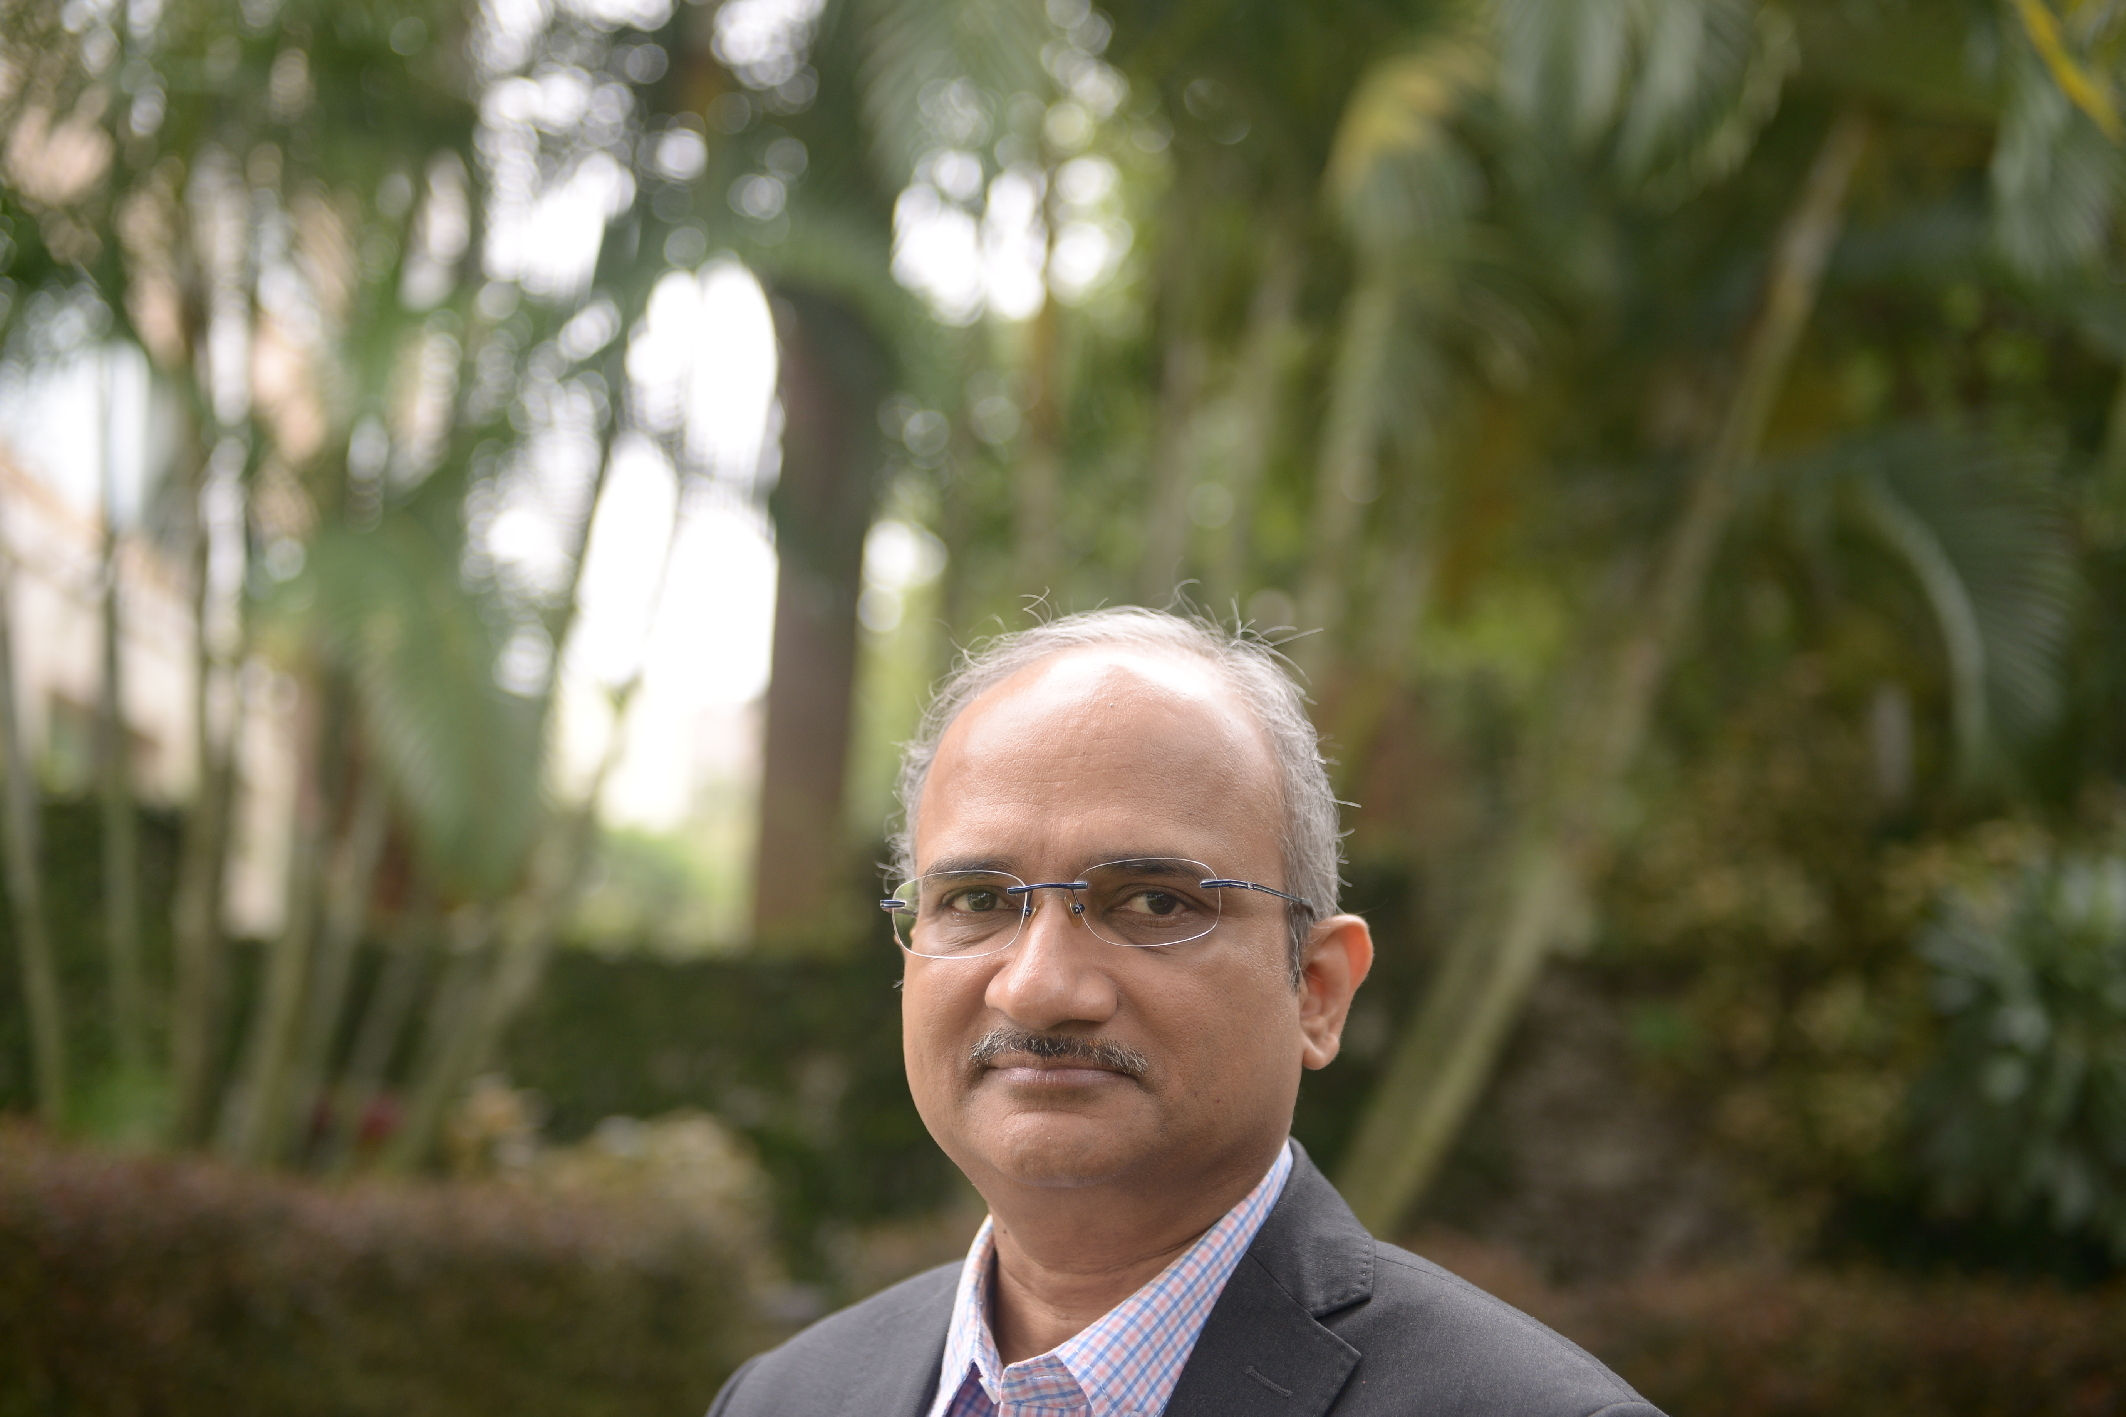
\includegraphics[scale=.5]{src/Figures/interview/interview-fig06.jpg}
\vspace{-.7cm}
\end{figure}

\textbf{\textit{RRV:}} No FinFETs are already there now. Every mobile phone, every chip that you see today that are 10 nanometer and 7 nanometer processors, they are all based on FinFETs. There are no conventional MOSFETs anyway. Our innovation was that while FinFETs often use SOI kind of processors which makes it easier in terms of processing, we tried to optimize the FinFETs for bulk applications.

That was a major contribution from our group. We tried to understand, optimize and then give directions to how these FinFETs instead of being on the SOI which is a very costly process can be integrated on bulk. We studied what sort of effects will come in and how can we alleviate those challenges.

We introduced lots of different concepts into the bulk FinFETs and that is a process now which everybody uses. In SOI it’s very simple but it’s expensive. In bulk it becomes a bit complex and there are lots of physical effects that take place which are unwanted. Now, the question is how do to integrate on the bulk process yet contain all of those effects that you see. That is where we introduced new concepts into FinFETs. We have patents for them as well.

\textbf{PH: Samsung seems to be talking about a version of FinFET which is the Gate All Around (GAA), so what do you foresee in the future?}

\textbf{\textit{RRV: }} That’s the next version. FinFETs have at least three side gates whereas the Gate All Around (GAA) kind of devices is the next thing that needs to happen if you want to contain the leakage currents, particularly the battery life. All of this from a consumer point of view translates into, say, how long the battery lasts, because the battery technology itself unfortunately is not keeping pace with the semiconductor technology.
 
 The mobile phones are becoming more and more capable, but the battery lasts hardly for a day even in the most modern kinds of devices. If you can innovate in terms of new battery technologies, then things would be quite great and the pressure on the semiconductor industries to improve the circuit performance will reduce a little bit.
 
 But since battery technologies are not keeping pace the semiconductor people must do a variety of things to reduce that standby power consumption and the GAA devices contain the short channel effects which leads to leakage of current. On-off ratios will get degraded and that is where the GAA will be very useful for the industry, but the process becomes much more complex.
 
 The question is: How do you put a gate underneath? Fabrication processes of embedding nanowires becomes more complex. Though FinFETs are now industry standard, going beyond making Gate All Around (GAA) will be a highly expensive affair and we haven’t as a community figured it out.
 
\textbf{PH: Right now, they are talking about 4 nanometers and 3 nanometers.}

\begin{figure}[H]
\centering
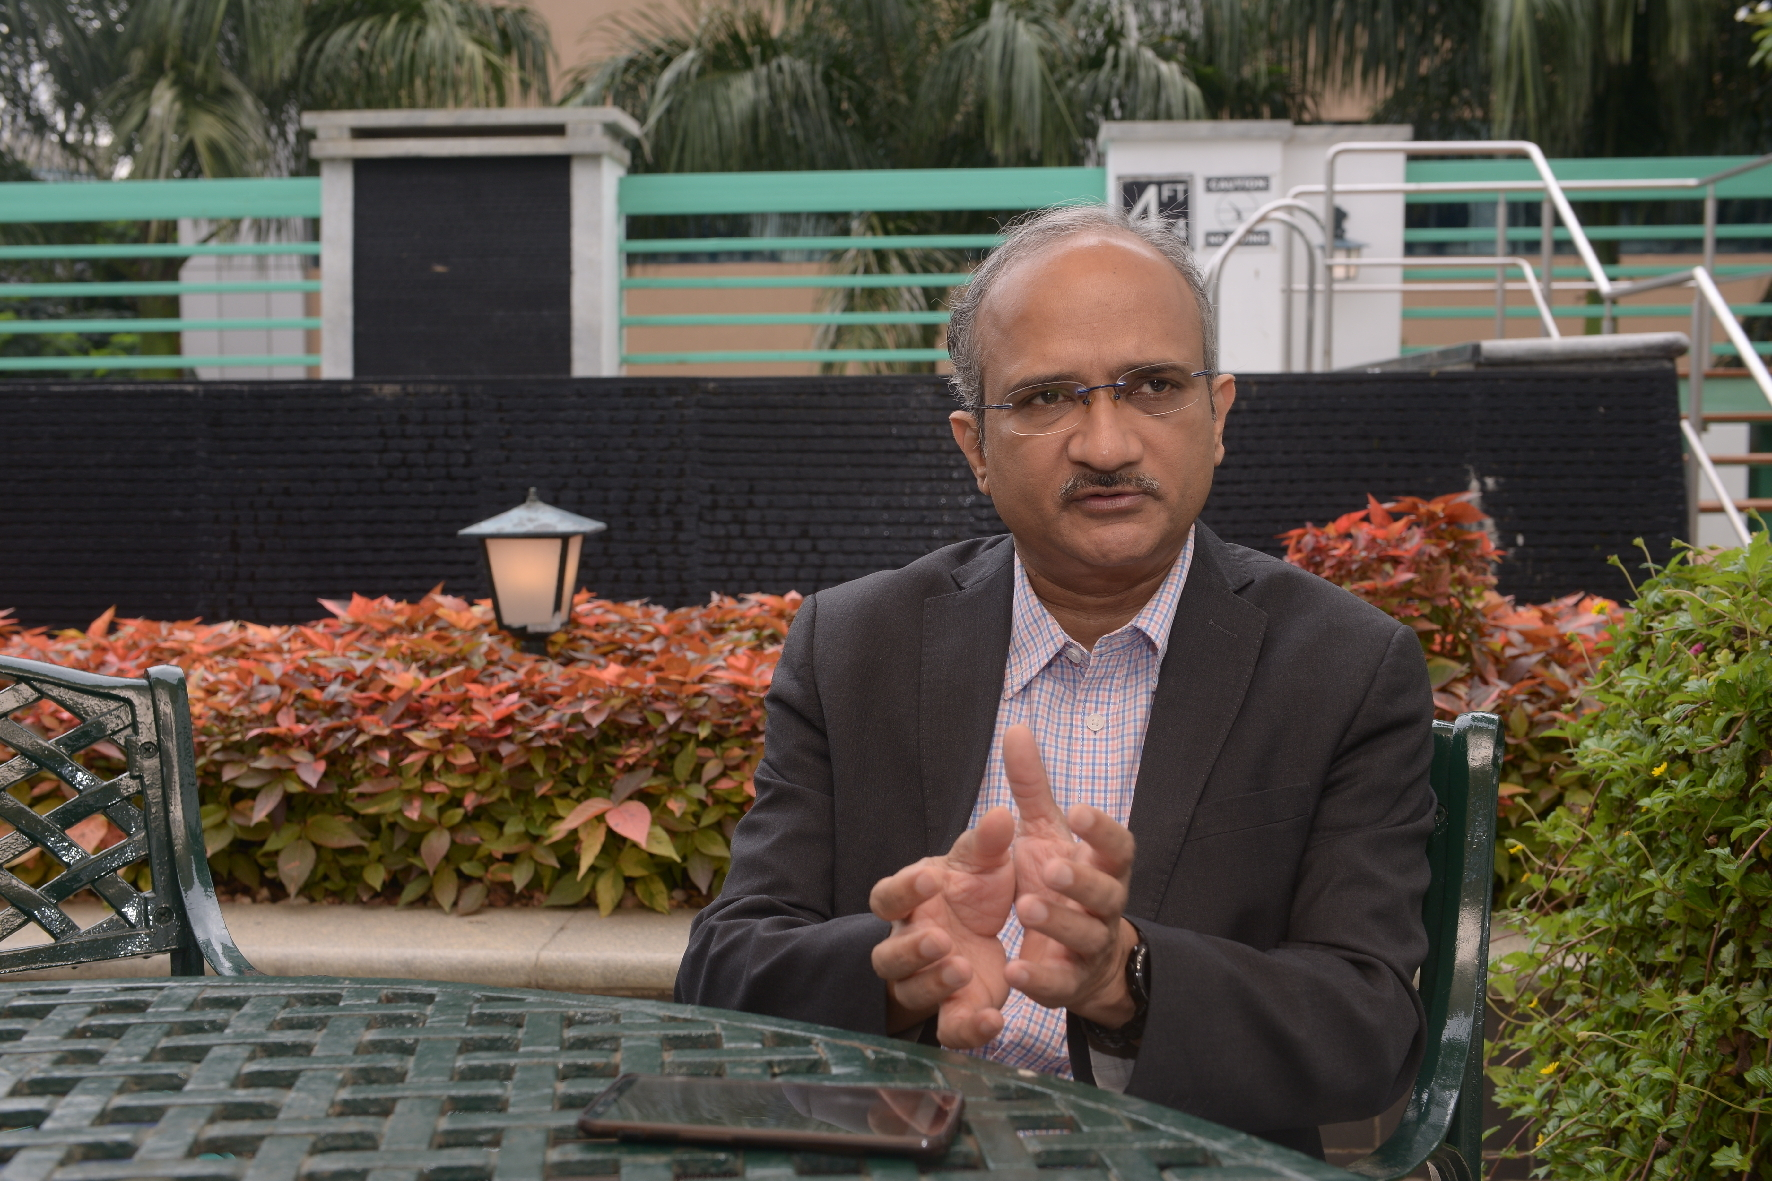
\includegraphics[scale=.59]{src/Figures/interview/interview-fig11.jpg}
\vspace{-.5cm}
\end{figure}

\textbf{\textit{RRV:}} Yes, there you need these nanowire kinds of devices that’s one-way and one-direction but for example the other way to reduce the standby power is to ask whether we can switch off the connection to the main power whenever a phone is in standby mode, where 80\% of your phone is really not doing anything. We have a project currently with Intel which is integrating mechanical switches with any electronic device that use MOSFETs in a logic operation like on-off states. We are exploring the idea of using nanomechanical switches that basically connects the chip to the main power and can effectively switch off or on during those logic blocks.

The question is how effectively can you cut them off from the battery and physically disconnect them and how fast can you do it?  You save completely on the power and the standby power but when you need to operate then it closes within a matter of a few nanoseconds or milliseconds or microseconds that the user wouldn’t even notice. So, integrating the nano electromechanical switches with the conventional CMOS is what we are exploring now. We have fabricated the switches and demonstrated them.

We have done a lot of work with Intel where we are modeling these switches along with the logic blocks and we have shown improvements in certain conditions where the duty cycles are very different. For example, the \textit{Off} time is very long and \textit{On} time is very short. For those applications it can give you tremendous advantages in terms of the standby power but where you have to continuously switch On and Off then it wouldn’t work much.

It’s turning out to be a very interesting idea. We developed the nanomechanical switch platform for our sensor work for explosive detection and other applications, but then we realized that it will also have applications here. The only change is if I am making it for sensors, I can use whatever process that works for me, but if I am trying to integrate with CMOS, then I am tied to whatever processes that are available in CMOS. So, integrating MEMS into a CMOS using the existing process flow is a challenge by itself and that is where we have lots of interesting collaborations with Intel.

\textbf{PH: Carbon has been touted for a long, long time now as an effective substitute to silicon. IBM seems to have done the 20 Nanometer experiment, where do you see this going?}

\textbf{\textit{RRV:}} With Carbon nanotubes control is the key, that is the major problem. The material looks good and everything is great but the fine control that you need to make these devices and integrate them into a billion transistor kind of a chip is not very easy. Carbon nanotubes though have been touted as things which will replace anything but I don’t see that happening. And that’s simply because of the control you need on the process for making it a mainstream kind of a technology is absent. As a material, Carbon nanotubes are used in many places but for CMOS applications using Carbon nanotubes is not going to be all that easy.

People are still exploring interconnect applications. The interconnects have become so complex and that kind of a fine control on Carbon nanotube process is missing. The other 2D material people are looking at is the Graphene. There again the band gap is zero so the Off currents are very high. And if you want to open a bandgap then the mobility is degraded therefore if you want to go for Graphene because of their high mobility, the leakage currents will become very high. And if you want to reduce the leakage currents by introducing a bandgap then the mobility suffers, so Graphene also has not been successful. There are basic issues with Graphene that people are not able to overcome right now. What IBM has shown is: In analog applications, can you use it instead of a logic gate where the On and Off operations are important? In an amplifier the transistor is never turned off. The transistor is always biased with a DC current and with the high mobilities you can achieve very high transconductances. So IBM and Samsung have shown Graphene based transistors for these very high frequency applications in the analog domain. So that’s a possibility that many industries are looking at but I think for an industry to change all these materials and go to something very new is not going to be easy. 

Whereas using the silicon using constrained engineering, using the channel with some of these materials with only a few layers of these materials going into the Gate All Around kind of a thing will happen one day or the other. And though there are new material introductions happening regularly in CMOS, I think currently the direction is not to continue to scale down the technologies.

These issues become very dominant and very prominent when you are scaling down. And the scaling down is not going to work too long. Parallelization is the approach now that everybody is taking. You will have multiple cores on the dye and the way the supercomputers are being built is how the processors are also being built in desktop computers and laptops and even in mobile phones with multiple cores. I think that is the way it will be and scaling this exponential kind of a growth cannot go on forever and everybody realizes it.

\textbf{PH:  So, you say that there is an imminent end to Moore’s law the way it is.}

\textbf{\textit{RRV:}} Moore’s law has already slowed down Now the scaling is no longer from a performance point of view and so I don’t think Moore’s law will survive for too long. It already has come to an end. But this parallelization is what is driving the current growth and power optimization is becoming very important. In fact, in a mobile phone what aspect of mobile phone you want to see as an improvement? It’s not the speed. I don’t think anybody is complaining of mobile phone speed. Everybody is complaining of the battery life. Though scaling improves the battery life it doesn’t solve the leakage currents problem which are becoming very high with scaling down. The scaling is not going to give you any further advantage in terms of battery life because of the short channel effects in the leakage currents. 

You can optimize the performance putting more cores on the dye which is a better approach. To me scaling has lived its life now. Now it’s time to look beyond scaling and integrate that more than more where you can have more sensors, more diverse technologies integrated, more diverse materials integrated. The brute force approach of scaling the device, I think, is the way to do it.

\textbf{PH: So Moore’s Law still lives in a parallel world.} 

\begin{figure}[H]
\centering
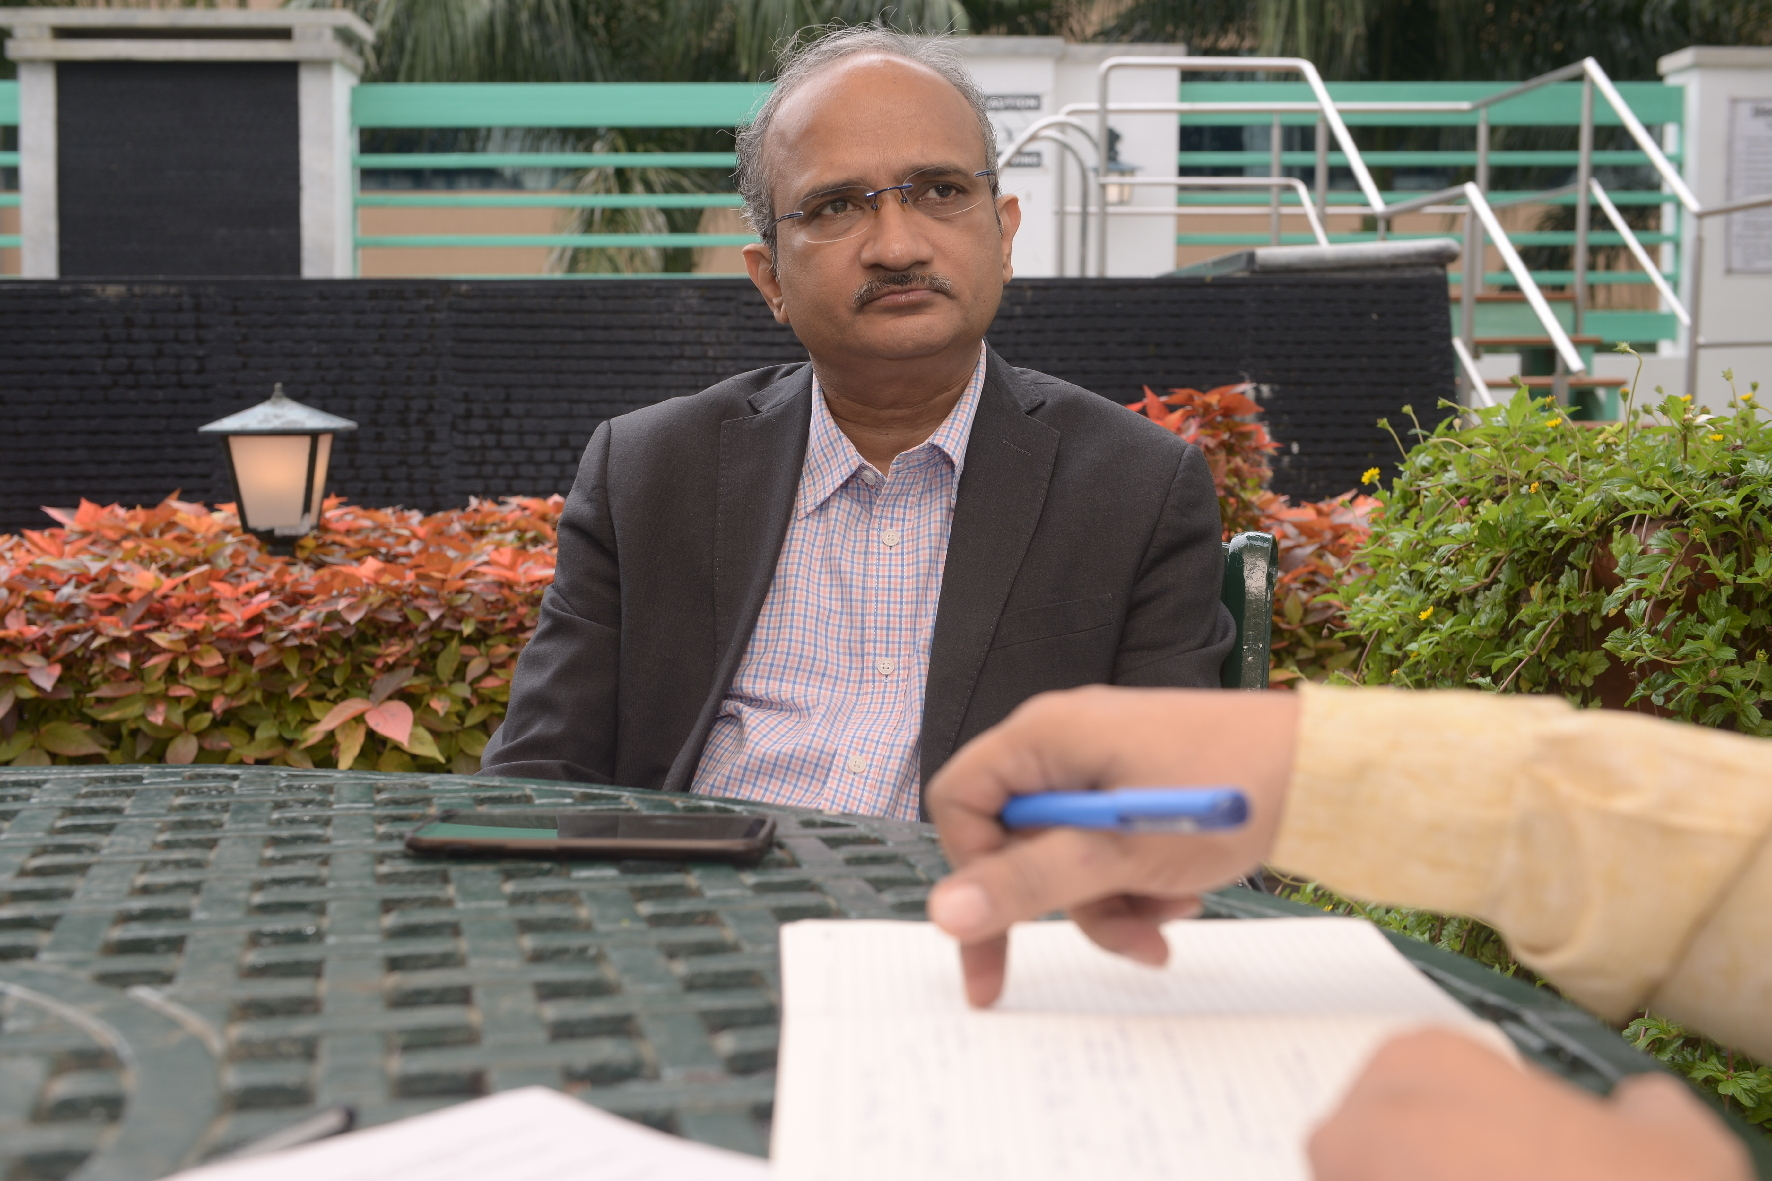
\includegraphics[scale=.59]{src/Figures/interview/interview-fig12.jpg}
\vspace{-.5cm}
\end{figure}

\textbf{\textit{RRV:}} Yes, in the parallel world and also the new material integration, the Systems on Chip kind of realizations. That will drive the future growth. So, as we talk about these IoTs and all of the sensors are going to be very, very important now and everybody focuses on the ICs but I think to me the bigger challenge is sensing.

The sensor technologies haven’t really evolved. It’s almost looking like, you know, the battery technology. They have not been keeping pace with the semiconductor industries because what can you sense today with enough accuracy? If I want to put right here multiple sensors and if I turn on the Bluetooth in my mobile, I should be able to know the air quality here.

Why are we not doing it? it’s not because the electronics is not there. The sensors are not available in most of the cases. Even where they are available the accuracies are not guaranteed. The specificity is not guaranteed. A lot of cross-talks in many of these sensors and the cost is are the big concerns. To put those sensors all around me, it will cost me so much of money. To me the sensor technologies is becoming a bottleneck for IoT, it’s not the IC the semiconductor technologies.

The sensors will require diverse kind of innovation, lots of new materials. If I want to sense a simple carbon monoxide (CO) I need to develop a material which doesn’t respond to CO2 but only responds to CO. I can tell you it’s not very easy.  And simple explosive detection you know there is no material which can only bind to the explosives and to nothing else because explosives also contain Hydrogen, Carbon, Nitrogen, Oxygen and it is also common in shoe polish, in perfumes and everywhere.

You need to do molecular recognition. This is not very easy and in Biology lots of nature designed processes which do molecular recognition exist but in synthetic areas, there is nothing where the molecules are recognized with enough accuracy.  Look at the antigens in the body, they recognize very specific targets and binding happens selectively, but they work only in the body. You take them out and they cannot even survive the normal temperatures -- these 30, 40 degrees kind of temperatures, many of these antibodies won’t even survive. We tried some of these approaches when we were looking at explosive detection. One of the ideas we tried with ITMEC in Chandigarh was to follow the nature’s approach to find selective receptors. So ITMEC scientists took these explosives [chemicals] injected them into animals and animals developed antibodies for these explosives. And they were able to extract those antibodies make a sensor out of it by coating these antibodies on surfaces in the external world and see if they can bind to the explosive.  The moment you bring these antibodies out of the animal ecosystem and put them on other surfaces they get denatured and doesn’t really work. They even tried to generate antibodies for explosives out of eggs as they are also living organisms.  Selectivity was always an issue and ITMEC is still pursuing some of those approaches. Nature does it routinely but when we try to create a synthetic kind of a thing there are too many cross-talks and cross-sensitivity issues which are a challenge.

And to me for IoT to take off we should be able to develop lots of new sensors which you can put them all over. Rest of the electronics part is easier and those things can be addressed. Today what you can sense are sight and sound. These we can do very well but can you smell things? No we cannot smell electronically yet. When it comes to smelling and taste, we have not captured the electronic nose electronic tongue platforms.  People are talking of it but I know the issues with selectivity, the training of these things is very difficult. We don’t actually know how our nose works and we don’t even know how our eyes see color despite all the understanding of human body. There are still a lot of things which we really don’t understand.

And to replicate the nature’s way on a chip is not going to be very easy and if you do the things become so complex the moment you start to mimic the nose because now I need to have a million sensors and then I need to have pattern recognition around these million sensors. It is not going to be as easy as it appears, while nature does it very effectively in the body but when you make million sensors now all these sensors need to be exactly identical and then when something binds the patterns I should be able to collect all the time in a very reproducible kind of a way which doesn’t work.

In Biology there is a lot of variability but there is also a lot of redundancy whereas when you try to capture it on a chip it’s very difficult to do all of that and so the problems become very complex if you are trying to mimic the nature but to me the sensor technology is a limitation and there is a huge scope for India to get into sensors.

I would like to see lots of government initiatives which are around sensor technologies because the moment you say sensors it comes into the natural sciences the physics and chemistry they become very important for developing the sensors. We have very strong Physics and Chemistry departments in the country.

So now if they can work with engineers and develop these sensors lots of great things will happen and DST has launched a major initiative where sensors is a major component in that.

We need to give more focus to the sensors and put India as a country which develops lots of these new sensors for new applications.  Sensors are going to be the future and even at IIT Delhi we started the center called Sense. 

It stands for Center for Sensors Instrumentation and Cyber Physical Systems with an acronym Sense and the latest thing we were trying to do was connect the engineering faculty with the Sense faculty.

Because many people in the Chemistry Department claim that lots of papers get written saying that I have been able to sense \textit{this and that}, they just remain as papers and engineers never really get to know them. But when engineers start to look at them and start to try them out, they don’t show the kind of claims that people make because they would test it under very controlled conditions.

But once you take it out into the field lots of things start to interfere which is a big challenge. What works for a sensor in the laboratory may not work the moment you take it but then that is where the engineers need to come in they need to work very closely with the science people so that you can improve things and further make them work outside. This calls for a very strong collaboration between the sciences and the engineering disciplines which is what we are trying to establish now.

I want to at least see a lot of focus given to the sensors area. The electronics part is under control all of us know the semiconductor industry is so advanced now and I think that part I am not worried but the sensors part is where I think there is a huge opportunity right now because people are talking of trillion sensor vision. Some people are saying that the number of sensors sold per year will reach a trillion kind of numbers in the next decade and even if you take \$1 per sensor it’s a trillion dollar market.

And you are talking of the entire semiconductor industry which is only 400 billion dollars or so to me it’s a huge opportunity for everyone.

\textbf{PH: In your ACCS-CDAC Foundation Lecture, you talked about how the receptors would not always bind and you fell back on another technique where you brought in Physics to replicating the explosion at a smaller scale, can you talk a little bit more about that?}

\begin{figure}[H]
\centering
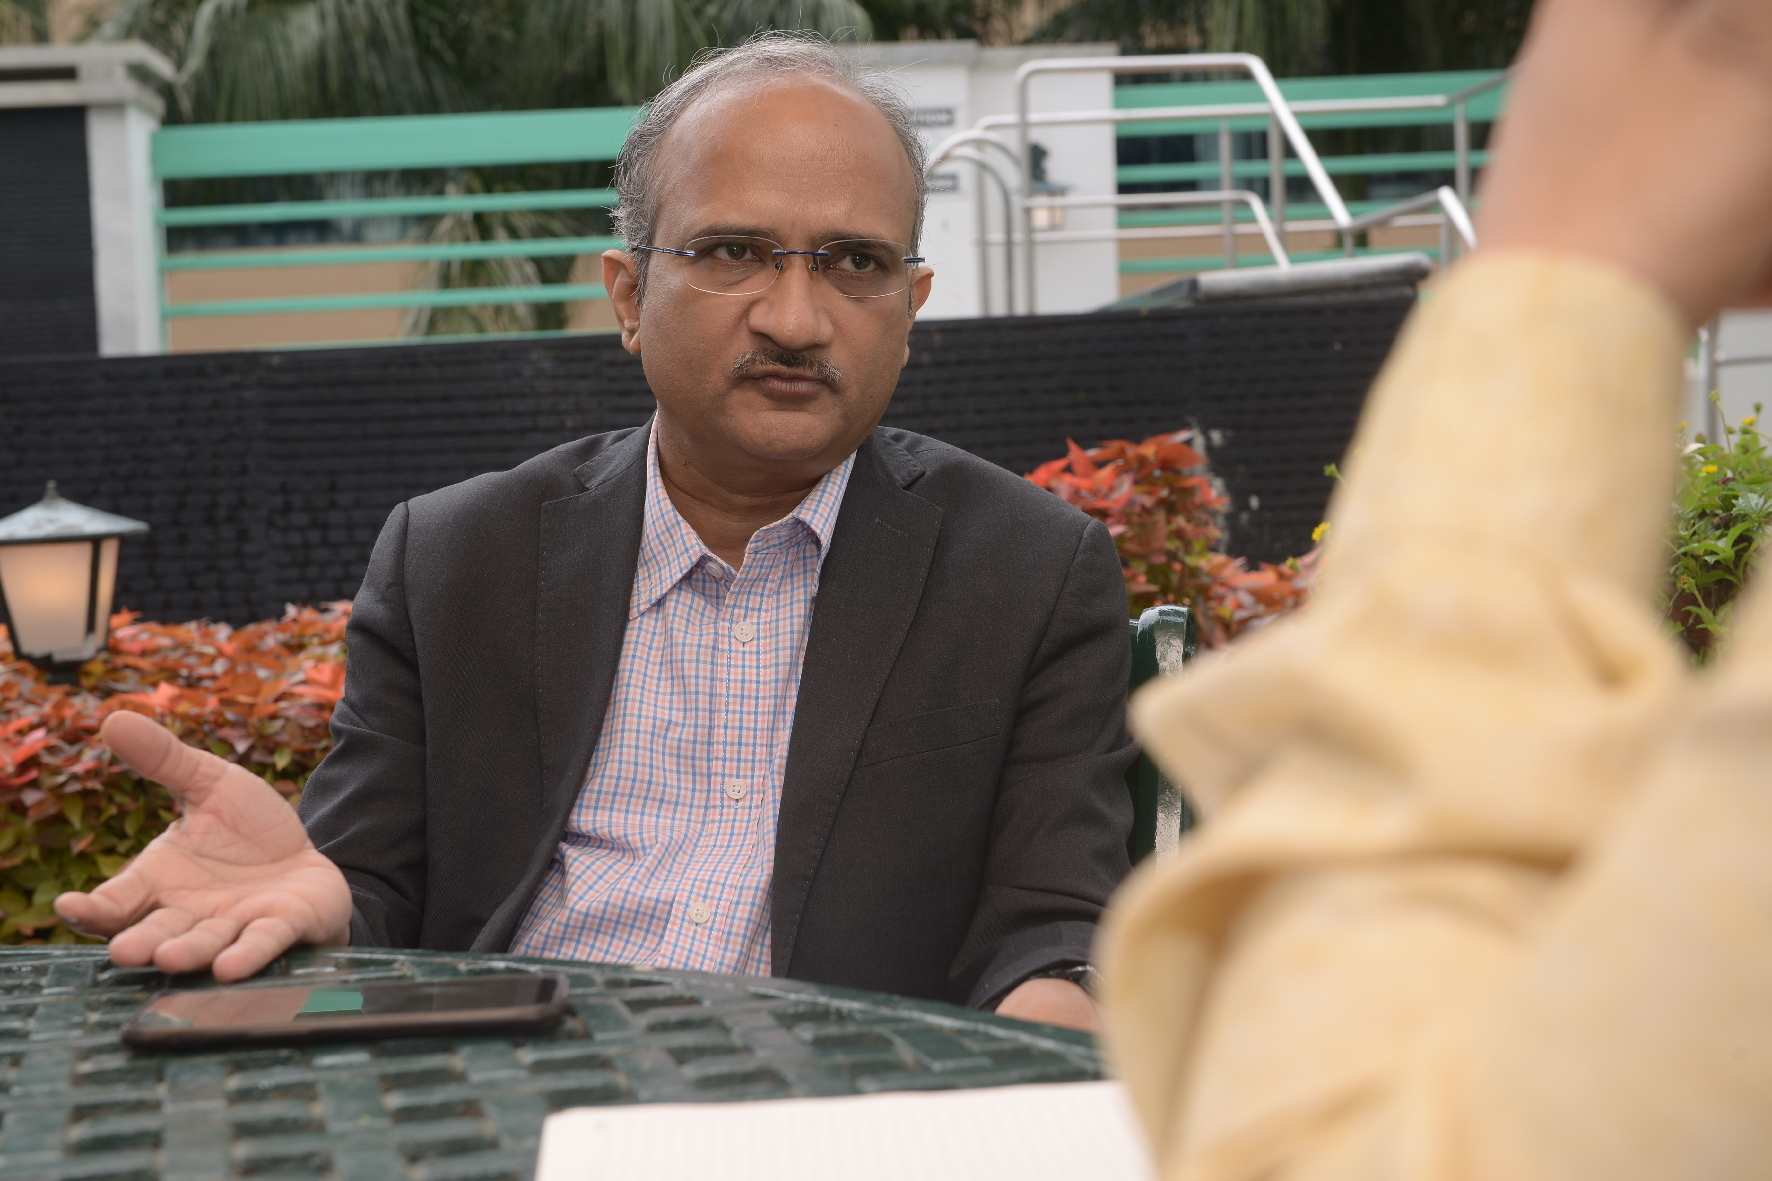
\includegraphics[scale=.59]{src/Figures/interview/interview-fig13.jpg}
\vspace{-.5cm}
\end{figure}

\textbf{\textit{RRV:}} Any binding host-guest kind of an event is never really very selective. I have tried quite a bit and it’s difficult to make anything work which is exactly selective to one particular thing under all conditions. In a controlled condition it is selective but the moment you put it under different conditions it tends to fail. That’s the reason why even simple fire extinguishers or the fire alarms do not work largely. We are not able to detect in fire in the $21^{\text{st}}$ century and now to be able to detect explosives selectively using those sort of approaches will still take consireable time.

\vskip -.2cm

At the end of the day the selectivity is a challenge for anything other than one or two parameters which we can measure right. But the Physics based approaches at least for explosives can be effective. Physics, as I was mentioning the way we were causing the nano explosions and detecting the event was an interesting approach. It works because Physics doesn’t depend on where you are testing it. Newton’s laws work everywhere it doesn’t matter where you are testing. I think that is the beauty of Physics.

\vskip -.1cm

\textbf{PH: So you would basically hold a library of behaviors of explosions, you do these explosions and match against the library, right?}

\textbf{\textit{RRV:}} Yes. Right now many of these sensors we are looking at it as yes or no. Is something an explosive or not an explosive? If somebody has a powder in the airport, I need to quickly know if it is explosive or not explosive. Today you need IMS kinds of systems which are very expensive. Each one of those is like \$25,000 to know whether that powder has any explosive kind of a thing.

That is the biggest challenge that the security agencies face and as a result they become paranoid they ban\break water and everything because they don’t know what is being carried about whereas with these technologies you can quickly tell whether something is an explosive or not.

\textbf{PH: And it is as good as the libraries that you are going to hold because there will be a lot of false positives.}

\textbf{\textit{RRV:}} Look at it this way, because only an explosive will explode, it doesn’t matter what that explosive is. So that way this approach will be qualitative but it will have at least 95\% kind of an accuracy. If you want to know what is that material then you need to do a lot of pattern recognition because every explosive event is different and now you need to train the system and all of that. That is a possibility one can look into but a qualitative way of knowing whether something is an explosive or not is possible now with a nano sniffer.

\textbf{PH: Since we are on the sensors I will jump over to that there is another point before I go that you talked yesterday you were talking about training the sensor using a library of data. Surprisingly you did not utter the word Machine Learning and Deep Neural Networks. Is it that you don’t want to use it or it doesn’t hold good in nanoscale? }

\textbf{\textit{RRV:}} No it is, it holds good but it’s a challenging problem. In fact, it needs a huge library. If I want to train for example at an airport put an electronic nose platform to detect explosives now what will passengers bring in the bags I need to train the system with all of that. So you need to generate a huge library of that for that but if I have just 4 sensors, I cannot have more than 16 possibilities for that because it will only give 0,0,0,1,2,1,1,1,1 these are all the patterns that I can have from 4 sensors now sixteen things it can detect by saying 10001 in one case 10000 in the other case but that won’t be sufficient because what can come inside the airport can be a huge number of things. 

If I need to increase my pattern size I need to increase my sensor’s size. The moment I increase it then the problem becomes complex and more difficult [to handle]. If somebody suddenly brings something [material] and the sensor doesn’t have it in the library it gives rise to speculation. One can use AI-MI kind of technologies to say that I don’t have a library but it looks something close to this kind of a thing.

I think the pattern recognition technologies will greatly benefit from the machine intelligence technologies for sure. But to me as a technologist the challenge is also on the hardware side. What can be the size of my chip, the sensor array and the larger I make it, the better it will be in terms of pattern recognition but the harder it will be to actually realize that and which is the challenge and therefore it’s a hardware software kind of a co design. And one can make it very complex in theory but the realization is a big challenge.

\textbf{PH: So, you are doing everything on the device, you don’t look at sending it out and getting the results.}

\textbf{\textit{RRV:}} In an airport kind of a thing you can have a small box which does everything which can be directly powered to the mains. So that is not a challenge for these technologies that way. But if you want to network them you cannot do. For buses, for example, the way we were looking at explosive detection is to place these sensors with limited power and they transmit when they recognize some event which is not looking really apt and the main processing can happen on a device connected to a power source.

\vskip -0.2cm

From the engineering point of view how much the sensor will do and how much you do in the backend is already solved. But the entire issue is with the sensors not with the electronics because electronics has advanced so much that we can do pretty much many things. The power source sometimes can be a big limitation. For example, for the application I was mentioning about explosive detector the power source is not very easy to build-in but we have done similar thing for agricultural sensors. We were able to put a solar panel on top because it’s always outside [in the Sun], it can benefit from the solar panel.  Energy harvesting kind of technologies from light to electricity can be done but from other means to convert that to electricity there are again material issues such as in the case of Piezoelectric. Why is it that from the motion and all that the human motion we are not able to power, say, the electronic watches? That is because efficiencies are very low and even if you can power it, it will be a few micro watts at the most and it doesn’t for the cost that it requires now and the complexity nobody is doing it.

\vskip -0.2cm

Otherwise in a simple electronic watch now this entire strap would have been your power generator. It’s not happening simply because those technologies are not there or they are very expensive. Where they are there the efficiencies are so poor that it doesn’t make any sense for anyone to do it today. That is the future for electronic watches -- the smart watches - where the battery is the biggest challenge by evening they become just some metal bands. The question there is can we use these energy harvesting technologies?

\textbf{PH: Just yesterday’s talk also just reminded me you know there used to be this gentleman called Greg Papadopoulos with Sun Microsystems long back in 2000 he was talking about internet dust with every spec having an IP of its own are we closer there? }

\textbf{\textit{RRV:}} It’s possible but to integrate it in that form factor is a challenge still. The future is all going to be whatever is science fiction today. Today’s science fiction will be a reality tomorrow. It’s a matter of integrating them and make them work for the kind of purpose that it is meant to perform. I think it will eventually happen.

\textbf{PH: But what challenges do you foresee in integrating these? }

\begin{figure}[H]
\centering
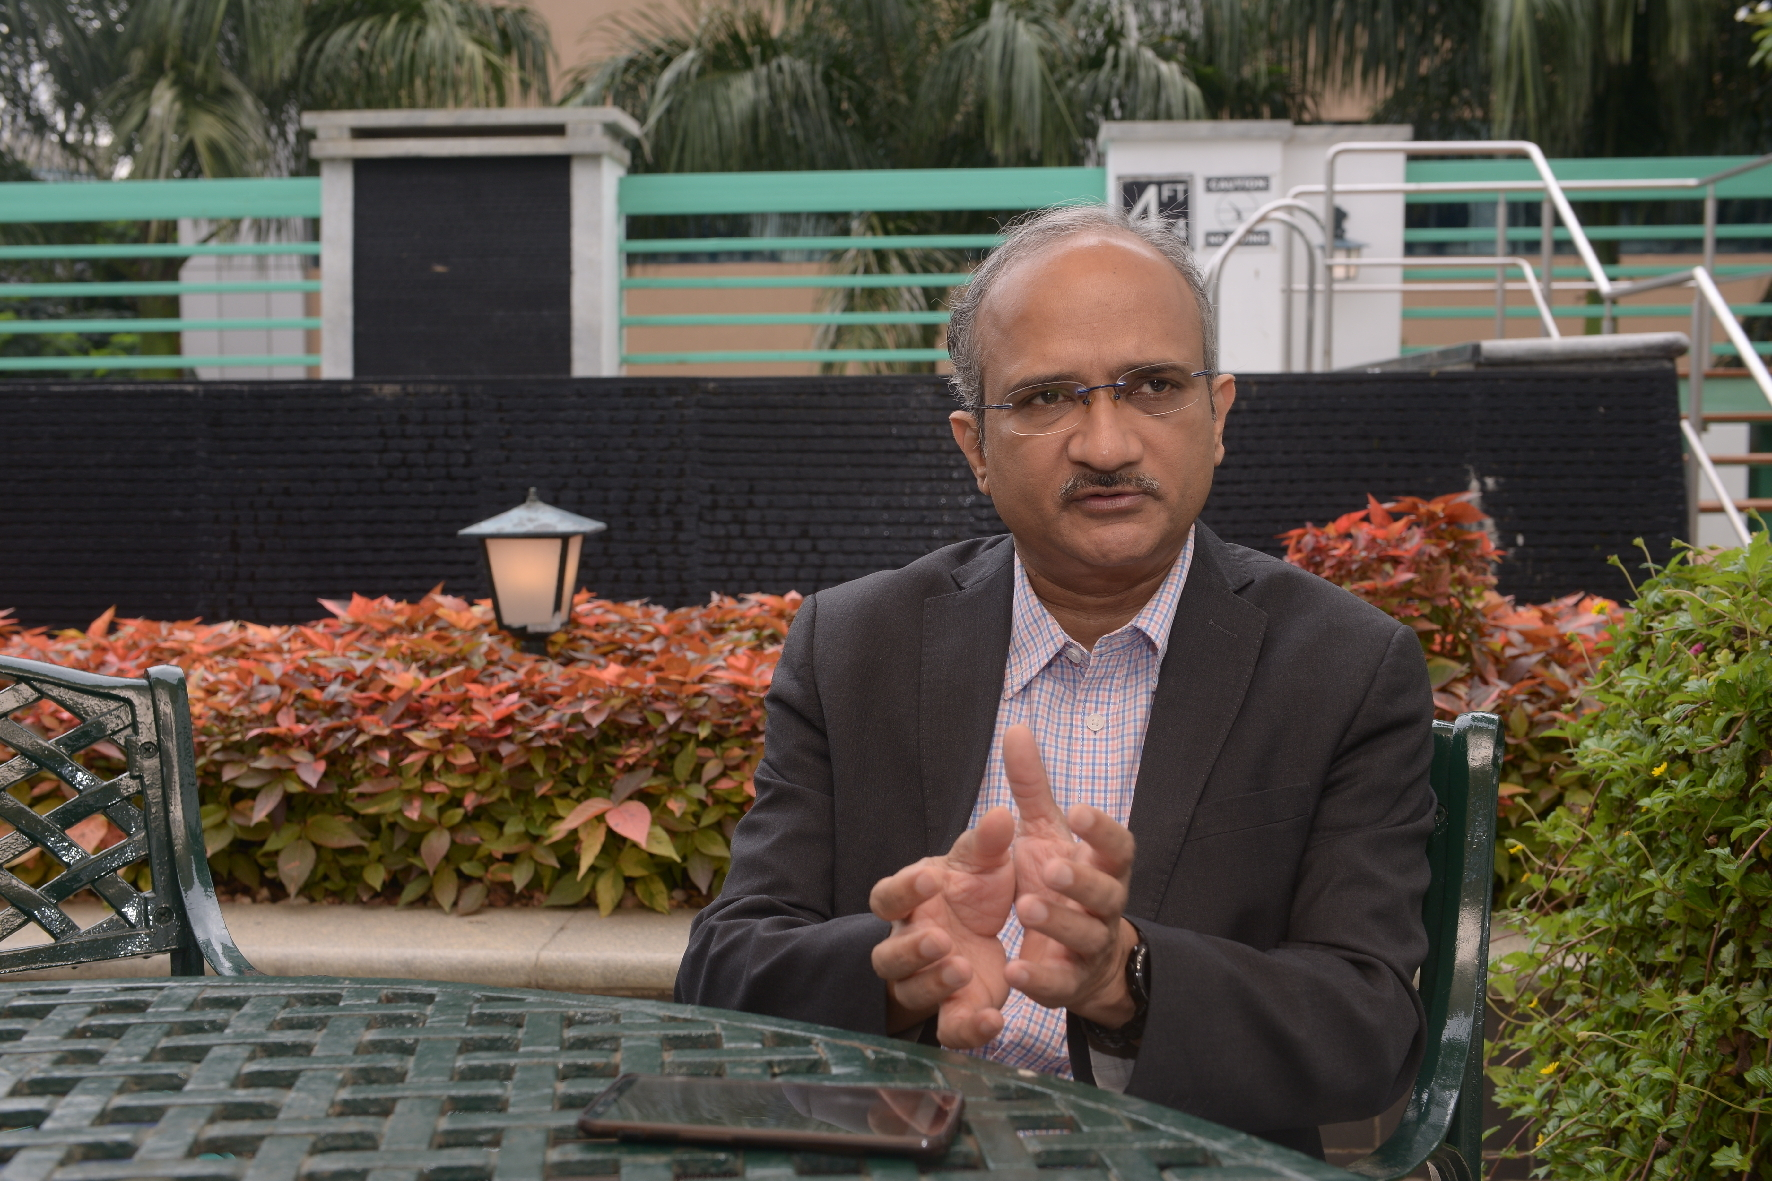
\includegraphics[scale=.59]{src/Figures/interview/interview-fig11.jpg}
\vspace{-.5cm}
\end{figure}

\textbf{\textit{RRV:}} Power, I think powering these sensors; developing these sensors you can put tiny cameras into those dust but then how will you power it? And that’s a challenge and if you don’t power it up by evening then the whole thing is dead. Energy harvesting to me is a very important area from powering point of view. We should be able to effectively harvest energy from all forms of sources that are available around us.

Today we can do to some extent the light to electricity or energy [conversion] but not with great efficiency. It would be 15\%, 16\%, 17\% [efficiency] which you can get commercially but that’s not much and that’s the reason why even simple solar cells are not taking off the way one would have expected. All those industries are losing money and that’s a challenge.

There are also so many other sources of energy, the microwave energy for example. There is so much of microwave radiation around us. Can you convert that microwave energy to charge the battery? That will require again technologies which will harvest microwave energy. It can be done but then you need the harvesters which themselves don’t consume power. Can you build these rectifiers which consume battery on their own? They have to be so efficient in terms of the conversion you can eventually gain something out of that. That conversion rates are not high today; efficiencies are not very high. 

\vskip -.2cm

As a result the energy harvesting other than from light to the electricity not other technologies are just not there. I can make a circuit put some PZT kind of material and have some LED bulbs glow, beyond that what have you done with energy harvesting? With Piezoelectric what applications do we see? There is so much of mechanical motion all around us, how much of it are we converting to electricity?

\vskip -.2cm

But the applications and the opportunities are huge and like I said if I want to have the IoT technologies in buses, trains and all those places, I think they need to find their own source of power. And wireless energy transmission to me is a great idea in fact that is what eventually will solve some of these problems when you enter  a home or enter a hotel there are wireless transmitters transmitting power and your battery everything is harvesting from there. 

\vskip -.2cm

Today the with the contactless chargers you don’t have to plug a wire into that you just place it on something and it charges but you take it one centimeter away then everything is gone. Now the future is all about charging from a distance and for that there will be lots of new technologies, new ways of doing things and there are some interesting possibilities.

\vskip -.1cm

\textbf{PH: So a philosophical question in a way we are looking at evolutionary nanotechnology rather than the so called revolutionary. I think the model that we have is ‘Honey I Shrunk the Kids’ that old… what kind of revolutionary nanotechnology do you foresee?}

\begin{figure}[H]
\centering
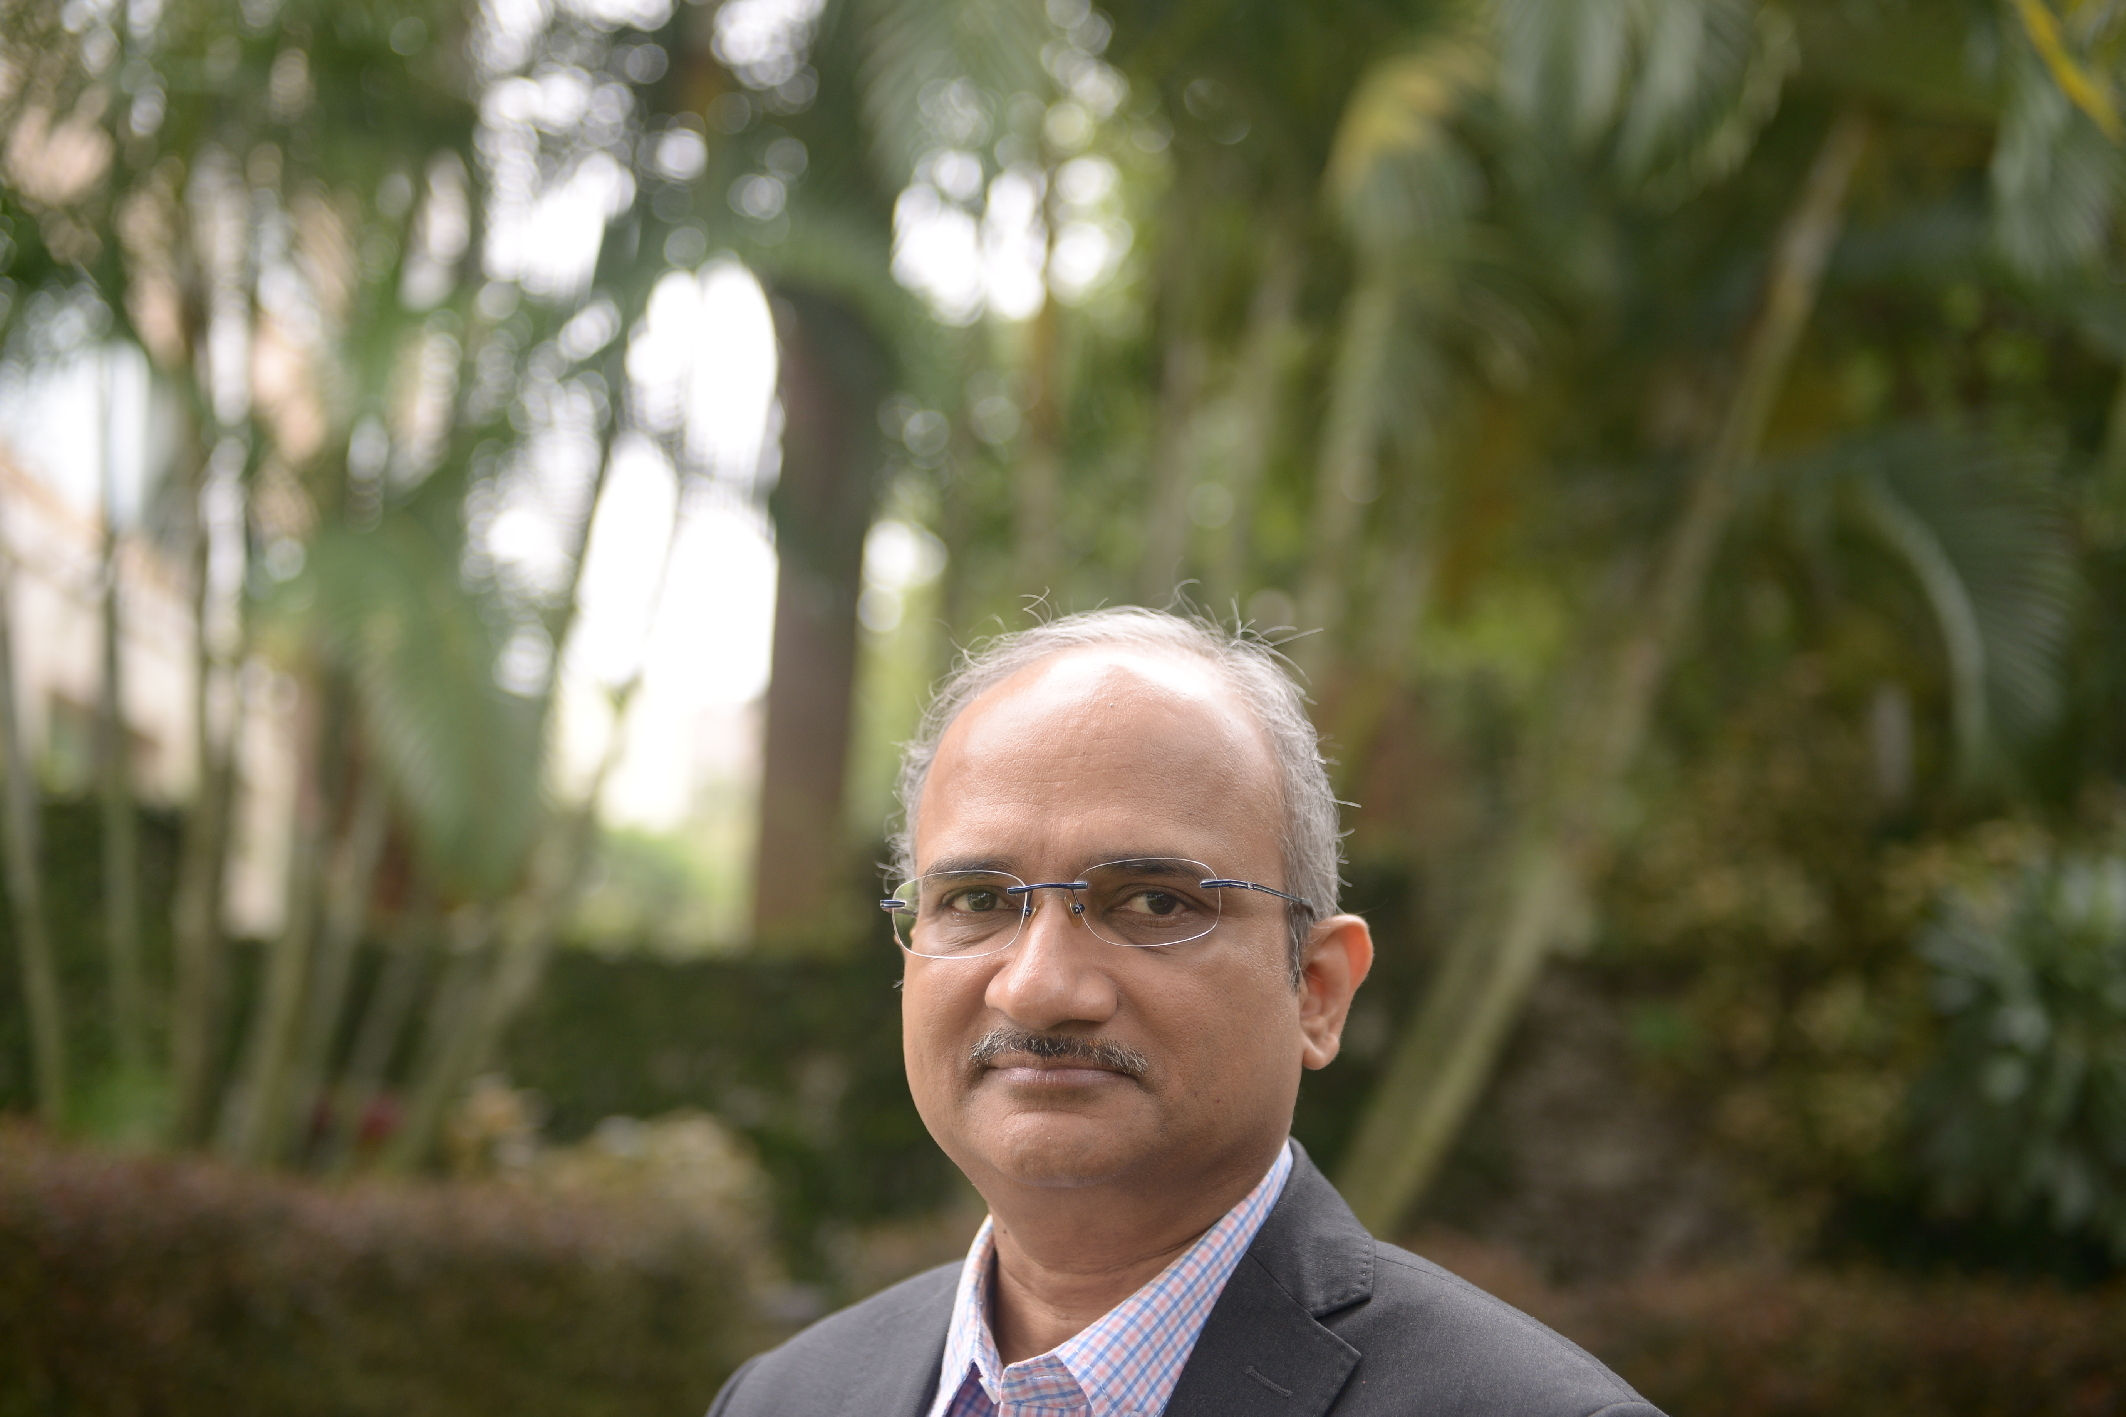
\includegraphics[scale=.5]{src/Figures/interview/interview-fig06.jpg}
\vspace{-.8cm}
\end{figure}

\textbf{\textit{RRV:}} In nanotechnology we are you know basically scratching the surface. The potential is huge and the issue is I think we are still doing it in a way where you make a material, you study properties and then you simulate to understand what you have found so that direction is what 99\% researchers are taking. But the reverse is we are playing God that I have this property of material; this is what I am looking for; can I reengineer materials to give me those properties? 

That is the revolutionary part and we are still not there. There are Nature papers trying to generate new materials but we don’t understand that. And at the molecular scale anything that you want to do becomes so complex you know first of all visualizing what is there in the molecular scale is through simulation. Even for a few molecules to simulate you need a supercomputer today. 

And things become very complex at the molecular scale and we are just nowhere close to playing God right now. It will take quite a bit of time and but even this normal evolutionary approach of you have a bulb material you make a nanomaterial, you characterize, you simulate and then you understand now what is happening I think that part once you go to nanoscale between what you characterize and what you simulate there is a huge difference right now. We don’t know what all is happening at the nanoscale which is giving rise to this new property. If I take a simple piezoelectric make it in the nano form what will happen to my piezoelectric properties? 

I can tell you to study that you need a supercomputer you need 100 people to actually do that. And so we attempted some of that we published some papers but we are all just scratching the surface and there is so much more to understand at the nanoscale. And that understanding will lead us to go through that revolutionary kind of a path and once this understanding is there then you can start to put it around and turn it around and say that I want these properties now this is the material I will create kind of a thing. I think but that is still a few decades away.


\textbf{PH: So that was my next question in fact in the classical world we have a playground where we know exactly what happens. Then we brought in the quantum physics now for nano and beyond you basically are saying that we still are not there.}

\textbf{\textit{RRV:}} We are just not there. I mean with some difficulty we are able to match the simulated characteristics with experimental characteristics you put in all the parameters that you have taken from experiments and you simulate and that simulation doesn’t match with the experimental data right now and we are still struggling to find out what else is happening and why is it not matching my calculation. That is where we are right now. 

And anything beyond that hopefully will happen one day but right now we are not there. 

\textbf{PH: Yeah so last couple of questions I think you are... So we were talking about... I want to go back to the multicore… see we have looked at software in a pretty... right from 1940 and we have not changed much only probably last ten years multicores have come and parallelization even today software cannot handle parallelization after certain cores. Now from your perspective, what is it that software engineers need to look at? We have talked about quantum computing, where are we headed?}

\textbf{\textit{RRV:}} See this is a hardware software co-design issue. I am not a software expert I am a hardware technologist but I also keep hearing that beyond a certain number of cores the software cannot handle it. And if we also think of it, the companies which are most valued in the world today are the ones which do their own software and hardware. If you look at iPhone what is the difference between Apple and Samsung?

Samsung is fitting their hardware into somebody else’s software so there are always some bugs that they face but what Apple does very effectively is they have their own designed hardware they have their own software therefore their interface is very smooth. I think that is the future. 

The same happens with Windows too the Microsoft thing. I think that hardware software codesign is going to give the users the better user experience. We have seen that we are seeing it everyday Apple kind of a thing. I think that is what probably the future will be and the software engineers need to work with hardware engineers. In fact, things are so bad today that even in microelectronics the device people, the technology people and the circuit people don’t talk to each other. And what the technologist would do what the device engineer would do what the circuit designer would do and because of that mismatch now there are huge kind of challenges.

A lot of my work has been in the circuit design device codesign. So we said technology aware design we started working in it with many industries. I have a gate all around kind of a transistor now if I want to design a circuit, circuit designer how much device background do I need to have to be able to effectively design gate all around kind of structures? 

And now this is a big challenge today even in FinFETs for example what should be the height of the Fin now who will decide what is the height of the Fin? Technologists will go by their technology considerations, the etching considerations to design the Fin but from a circuit designer point of view, is it optimum? If I increase the height of the Fin, the total width of my transistor will increase.

But you know for many transistors I don’t want that large width it will only consume my battery so the... but then for the FinFET designer to work with a circuit designer and design what is the optimum height for the Fin though it looks very natural but it’s so difficult to implement it in the real kind of a fashion because they speak completely different languages.

\vskip -.2cm

So that is a challenge today even in the same industry microelectronics industry bringing technology design device and the circuit people together is a big issue right now and I can write papers even by looking at simple you know nanowire transistors and designing a circuit with nanowire transistors those papers get accepted anywhere just like that because there are so few papers which talk about the nanowire to the circuits kind of a thing they all stop with the devices.

\vskip -.2cm

To go from devices to circuits is a big challenge today and in that scenario now to bring to make software guys to work with the hardware guys because they are all in their own silos is again a big challenge. And the companies which have been able to do it effectively are the world leaders today. I think that is what is required from the optimization point of view these silos need to be broken. There should be people who can talk the device language and also the circuit language and also the technology language.

\vskip -.2cm

Most of my students are very valued and joined industries and are doing very well because of the technology aware design areas we worked on. They could speak circuits with the same confidence as they can discuss the devices the technologies. So that is a very valuable sort of an expertise many of my studentspossess. They are all doing very well right now because of that.

\textbf{PH: Now my last question Quantum Computing we have been hearing of this for quite some time but there seems to be some basic theoretical hurdles, conceptual hurdles for it to really come into the mainstream, what is your view?}

\textbf{\textit{RRV:}} Again I don’t work in the Quantum Computing area but just my perception about Quantum Computing is I think now things are taking off I think all these the security the cryptography and all of that I am told Quantum Computers are much more effective than the\break normal computers and you can use them on the cloud already. And I think a lot of advances happened in the last 5 years and India has missed that bus again as usual simply because in India now with governments and everybody asking for technologies and what is the outcome, what is all of this we are not spending enough on the basic research.

And Quantum kind of areas have always been seen as some blue sky research which you know which India cannot afford or we should be connecting all our research to societal problems. In the process we never invested enough in the basic research. As a result, in the country today I cannot even name five groups which are doing any great work in Quantum Computational areas which is a pity now for a country like India and we have now missed that bus which is bad because anything... In fact, I keep telling this everywhere that if we only focus on technologies the technologies evolve out of basic research.

Even simple things like the gravitational wave is as basic research as a technology research. Why do we need to study what is happening in the universe somewhere far away but if you actually think of it what the gravitational waves have done is until now you could only visualize the sky or the universe by observing with all these huge telescopes we were able to see and do all of that. But what gravitational waves have given us another way to probe the universe and soon that will become a technology by itself. And as a result, what looked like a very basic fundamental blue sky research will start to have applications and it will change astronomy because I have another way to look at the universe and that is what we’ll do.

Today’s basic research is tomorrow’s technology and if we only focus on technology, then you are cutting off that pipeline that you know after sometime you will have nothing to work on. And that is what has happened with Quantum Research because government is not willing to give money for basic research. I think we always have in the country the resources were always limited and whatever resources we had because of pressure from every quarter we invest in technologies which can immediately result in something, but in the process we have cut down that pipeline.

We have throttled that pipeline that now we don’t have enough basic research happening which can feed\break tomorrow’s technologies. And as a result the Quantum Computing is one great example. The world persisted, the US kind of countries persisted; after 30 years, 35 years now you are seeing the application of those Quantum Computers.

And it takes that long for a great idea to become something which is worthwhile. These are things we are not managing. We are not investing enough in our science which is the basic problem right now. We must increase our spending on academic research from 0.6, 0.7 percent GDP to least three times. Today’s blue-sky research will be tomorrow’s basic technology kind of a platform.

To get a Nobel prize, you need to identify 25 groups in the country and fund them with whatever they need. And then you wait for 10, 15, or even 20 years for them to eventually make a mark on the world stage. We are not doing that. For me, even to get a 15 lakh consumable, I need to run to DST (Department of Science and Technology) and write a proposal, wait for 6 months to get that 15 lakhs.

I think with that sort of a thing and such an ecosystem that we have built in this country, Nobel prizes will not happen. So for that to happen, you have to identify 25 top groups and give them whatever they require. And don’t even ask them any questions for 15 years or 20 years kind of a thing so out of that we will generate next generation Nobel Laureates. We are not doing it right now. We are becoming \textit{penny-wise pound-foolish} kind of a thing and everybody is asking for immediate returns. I have given you this money where is your result, where is the prototype and where have you tested? These questions science cannot work like that.\hfill \raisebox{-.1cm}{
\includegraphics[scale=.9]{src/Figures/circledC.eps}}
\end{multicols}
